% =====================================================================
% Supplementary Information for Paper E1 v69
% Does a surplus-production ladder improve forecasts of Northern cod?
% =====================================================================
\documentclass[preprint,11pt,authoryear]{elsarticle}
\usepackage{amsmath,amssymb,amsthm}
\usepackage{booktabs}
\usepackage{array}
\usepackage{tabularx}
\usepackage{longtable}
\usepackage{graphicx}
\graphicspath{{./}{figs/}{paperE1_cod_forecast_ladder_v69_src/figs/}}
\usepackage{enumitem}
\usepackage{placeins}
\usepackage[colorlinks=true,urlcolor=blue,linkcolor=blue,citecolor=blue]{hyperref}
\emergencystretch=3em
\setlength{\tolerance}{2000}
\renewcommand{\topfraction}{0.9}
\renewcommand{\textfraction}{0.07}
\renewcommand{\floatpagefraction}{0.75}

\renewcommand{\thesection}{S\arabic{section}}
\renewcommand{\thetable}{S\arabic{table}}
\renewcommand{\thefigure}{S\arabic{figure}}
\renewcommand{\theequation}{S\arabic{equation}}
\theoremstyle{remark}
\newtheorem{remark}{Remark}
\renewcommand{\theremark}{S\arabic{remark}}

\newcommand{\kt}{\,\mathrm{kt}}
\newcommand{\Blim}{B_{\mathrm{lim}}}
\newcommand{\RMSE}{\mathrm{RMSE}}
\newcommand{\sA}{\mathfrak{s}}
\newcolumntype{L}{>{\raggedright\arraybackslash}X}

\journal{Fisheries Research}

\begin{document}

\begin{frontmatter}
\title{Supplementary Information for:\\ Does a surplus-production ladder improve forecasts of Northern cod? A scored retention test against persistence on NAFO 2J3KL}
\author[1]{Amin Abaee\corref{cor1}}
\ead{amin_abaee@ut.ac.ir}
\cortext[cor1]{Corresponding author. ORCID: 0000-0002-0019-1842.}
\affiliation[1]{organization={Independent Researcher}, city={Tehran}, country={Iran}}
\begin{abstract}
This Supplementary Information records the material that supports the main text without carrying its argument: the pass order and protocol status (S1); the origin sets (S2); the full Diebold--Mariano and paired block-bootstrap grids with block-length sensitivity (S3); the period decomposition at five years, on the annual-landings pass, and the post-1995 pooled margins with intervals (S4); the fitted parameters of every fixed window and every rolling origin (S5); the census of floor forecasts (S6); the secondary scores (S7); the simulation design, the power decomposition, the chance baseline, the alternative rules and the failed pre-check diagnostics (S8); the decomposition of the lagged-start module's deficit (S9); the Edwards Aquifer restatement of the rule (S10); the vintage and threshold comparisons (S11); the 2022--2023 observation-suspension chronology (S12); the reproducibility and verification record (S13); and the catch-timing sensitivity (S14). Section, table and figure numbers without the prefix ``S'' refer to the main text.
\end{abstract}
\end{frontmatter}
\section{Pass order and protocol status}\label{si:passes}

The study is a fixed computational protocol with a recorded execution order, not a prospective registration: no dated pre-scoring protocol file exists for the empirical passes. The order below is established from the analysis code and its archived metadata. Passes 1 and 2 are labelled in the driver script \texttt{run\_ladder.py} and distinguished in \texttt{results/meta.json} by the keys \texttt{catch\_pass1} and \texttt{catch\_pass2}; passes 3 and 4 are separate scripts that import from that driver, which fixes their order after it.

\begin{table}[!htb]
\centering\small
\caption{Order in which the passes were run.}
\begin{tabularx}{\textwidth}{@{}clLL@{}}
\toprule
\# & Pass & Data treatment & Script / archived output \\
\midrule
1 & Coarse-regime catch & 240/120/5\,kt (through 1991 / 1992 / from 1993) & \texttt{run\_ladder.py} (pass 1); \texttt{fixed\_window\_scores.csv}, \texttt{rolling\_summary.csv} (rows \texttt{catch = regime}), \texttt{rolling\_forecasts\_regime.csv} \\
2 & Annual landings & Schijns et al.\ (2021) Table 1, t/1000 & \texttt{run\_ladder.py} (pass 2); same files, rows \texttt{catch = annual}; \texttt{rolling\_forecasts.csv} \\
2b & Survey start & Forecast initiated at the survey-scaled state, annual catch & \texttt{run\_survey\_start()} within pass 2; \texttt{survey\_start\_forecasts.csv} \\
3 & Capelin variants & Two-regime $r$ at the 1991 break; acoustic-index multiplier on observed years & \texttt{run\_capelin\_regime.py}, \texttt{run\_capelin\_index.py}; \texttt{capelin\_*\_summary.csv} \\
4 & Specification B & The ladder on the xteNCAM series alone, not pooled & \texttt{run\_xte.py}; \texttt{xte\_rolling\_summary.csv}, \texttt{xte\_fixed\_window\_scores.csv} \\
5 & Uncertainty layer & DM statistics and block bootstrap on the archived per-origin files & \texttt{campaign\_e1\_dm\_uncertainty\_regime.py}; \texttt{e1\_dm\_uncertainty\_regime.csv} \\
6 & Simulation & D1--D5 per \texttt{SPECIFICATION\_v4.md} (locked 2026-09-10 before the code was written); D6--D7 per Amendment 1 (locked 2026-09-11) & \texttt{tools/sim\_retention\_power.py}; \texttt{sim\_retention\_power.csv}, \texttt{sim\_misspecified\_D6D7.csv} \\
7 & This revision & Re-execution of passes 1--6 in a third environment; paired bootstrap confirmation; period decomposition; rolling parameter record; catch-timing sensitivity & \texttt{paperE1\_cod\_forecast\_ladder\_v69\_src/work/} in the repository \\
\bottomrule
\end{tabularx}
\end{table}

Three points bear on how the scores should be read. The five ladder modules were fixed before any pass was scored: the \texttt{SPECS} list in \texttt{run\_ladder.py} defines M1, M1b, M2, M3 and M4 once, Specification B imports that list rather than redefining it, and none was altered after a score was seen. The scoring core, the fixed windows, the rolling-origin RMSE comparison and the persistence bar at both horizons, was coded before the first pass. Two elements of the retention rule were formalised after the pass-1 scores had been computed: the 5\% tie band and the comparator declarations for the non-nested modules (M2 against M1, M4 against M3). Neither decides any retention outcome, the smallest pooled deficit against persistence being 17.1\%. The capelin pass is the one place where a model was added after scoring began (the index multiplier), and it is reported as a variant, not as a member of the ladder. Specification B was run last and never pooled with Specification A; the constraint is recorded in the code's docstring and in \texttt{meta.json}.

\section{Origin sets and windows}\label{si:origins}

\begin{table}[!htb]
\centering\small
\caption{Origin sets. All baselines are evaluated on the module's own origin set at each horizon. The mixed-origin persistence values that the archived Specification B summary also carries (87.6 and 317.7\,kt on 63 and 59 origins) are not comparators and are not used.}
\begin{tabularx}{\textwidth}{@{}>{\raggedright\arraybackslash}p{0.36\textwidth}Lcc@{}}
\toprule
Pass & Origins & $n$ ($h=1$) & $n$ ($h=5$) \\
\midrule
Specification A, ladder (all catch passes, survey start, two-regime $r$) & 1990--2014 ($h=1$); 1990--2010 ($h=5$); minimum eight training years & 25 & 21 \\
Specification A, capelin-index multiplier & 1991--2014; 1991--2010 (origins with a carried acoustic value) & 24 & 20 \\
Specification B, ladder and two-regime $r$ & 1965--2023; 1965--2019; minimum twelve training years & 59 & 55 \\
Specification B, capelin-index multiplier & 1988--2023; 1988--2019 & 36 & 32 \\
\bottomrule
\end{tabularx}
\end{table}

The capelin acoustic index is observed in 1982 and 1985--2023 with gaps (1983, 1984, 1993--1995, 1997, 1998, 2006, 2016, 2020--2022 missing; 2023 $= 331.3\kt$). The multiplier pass carries the last observed value across gaps and drops origins with no carried value; the two-regime pass uses the 1991 capelin collapse as a declared break and allows $r$ to differ before and after it, with the post-break value estimated only once post-break transitions are in the training window.

\FloatBarrier
\section{Uncertainty layer: full grids}\label{si:uncertainty}

Table~\ref{tab:si_dm} gives every module--benchmark pair of the archived uncertainty layer: the DM statistic (loss differences of squared errors; autocorrelation-consistent variance truncated at lag $h-1$; reported as a $z$-score), the paired moving-block bootstrap interval of the RMSE gap (block $\max(h,3)$, 20\,000 replicates, seed 0) and its two-sided $p$-value. The bootstrap in the archived script draws block indices from a generator seeded identically for the two loss series, so the resample is paired; re-running it with an explicitly shared index draw reproduces every interval to the printed digit. Table~\ref{tab:si_blocks} gives the block-length sensitivity (5\,000 replicates per cell) for the M1 and M3 persistence margins.

\begin{table}[!htb]
\centering\scriptsize
\setlength{\tabcolsep}{3.5pt}
\caption{Archived uncertainty layer: all pairs. RMSE in kt; gap $=\RMSE(A)-\RMSE(B)$; CI is the 95\% paired block-bootstrap interval of the gap; $p$ is the two-sided bootstrap $p$-value. The M2-against-M1b rows are an alternative-comparator disclosure, not part of the rule.}
\label{tab:si_dm}
\begin{tabular}{@{}ccllrrrrrlr@{}}
\toprule
Spec. & $h$ & A & B & $n$ & RMSE(A) & RMSE(B) & gap & DM $z$ & 95\% CI & $p$ \\
\midrule
A & 1 & M1 & persistence & 25 & 120.5 & 98.0 & +22.5 & 1.13 & [-13.4, +52.2] & 0.19 \\
A & 1 & M1b & persistence & 25 & 114.8 & 98.0 & +16.8 & 0.98 & [-19.4, +59.6] & 0.38 \\
A & 1 & M2 & persistence & 25 & 144.1 & 98.0 & +46.0 & 1.29 & [-12.3, +83.0] & 0.45 \\
A & 1 & M3 & persistence & 25 & 134.6 & 98.0 & +36.6 & 0.99 & [-16.8, +64.2] & 0.93 \\
A & 1 & M4 & persistence & 25 & 195.6 & 98.0 & +97.5 & 1.53 & [-9.1, +172.7] & 0.28 \\
A & 1 & M2 & M1 & 25 & 144.1 & 120.5 & +23.5 & 0.91 & [-60.7, +66.9] & 0.68 \\
A & 1 & M4 & M3 & 25 & 195.6 & 134.6 & +60.9 & 1.21 & [+4.4, +134.4] & $<0.005$ \\
A & 1 & M2 & M1b & 25 & 144.1 & 114.8 & +29.3 & 0.91 & [-67.6, +82.8] & 0.70 \\
A & 5 & M1 & persistence & 21 & 288.7 & 264.7 & +24.0 & 1.84 & [-43.1, +56.4] & 0.28 \\
A & 5 & M1b & persistence & 21 & 288.6 & 264.7 & +23.9 & 1.84 & [-43.1, +56.4] & 0.28 \\
A & 5 & M2 & persistence & 21 & 398.2 & 264.7 & +133.5 & 1.10 & [-21.0, +217.5] & 0.42 \\
A & 5 & M3 & persistence & 21 & 366.4 & 264.7 & +101.6 & 1.12 & [-0.8, +151.4] & 0.08 \\
A & 5 & M4 & persistence & 21 & 488.2 & 264.7 & +223.5 & 1.14 & [-20.8, +409.4] & 0.40 \\
A & 5 & M2 & M1 & 21 & 398.2 & 288.7 & +109.5 & 0.98 & [-77.1, +232.8] & 0.81 \\
A & 5 & M4 & M3 & 21 & 488.2 & 366.4 & +121.9 & 1.15 & [-27.4, +263.2] & 0.71 \\
A & 5 & M2 & M1b & 21 & 398.2 & 288.6 & +109.7 & 0.98 & [-77.1, +232.8] & 0.81 \\
B & 1 & M1 & persistence & 59 & 119.5 & 84.4 & +35.0 & 2.81 & [+2.7, +70.8] & 0.03 \\
B & 1 & M1b & persistence & 59 & 151.6 & 84.4 & +67.2 & 3.60 & [+18.3, +117.7] & 0.01 \\
B & 1 & M2 & persistence & 59 & 166.0 & 84.4 & +81.6 & 3.22 & [+36.4, +122.8] & $<0.005$ \\
B & 1 & M3 & persistence & 59 & 126.7 & 84.4 & +42.3 & 1.85 & [+1.0, +92.5] & 0.04 \\
B & 1 & M4 & persistence & 59 & 205.7 & 84.4 & +121.3 & 3.20 & [+53.7, +193.0] & $<0.005$ \\
B & 1 & M2 & M1 & 59 & 166.0 & 119.5 & +46.6 & 1.78 & [-20.5, +104.5] & 0.17 \\
B & 1 & M4 & M3 & 59 & 205.7 & 126.7 & +79.0 & 3.07 & [+35.6, +116.4] & $<0.005$ \\
B & 1 & M2 & M1b & 59 & 166.0 & 151.6 & +14.4 & 0.51 & [-67.5, +89.1] & 0.77 \\
B & 5 & M1 & persistence & 55 & 431.9 & 300.0 & +131.9 & 2.06 & [+33.2, +218.6] & 0.01 \\
B & 5 & M1b & persistence & 55 & 445.5 & 300.0 & +145.5 & 1.80 & [+18.2, +250.9] & 0.02 \\
B & 5 & M2 & persistence & 55 & 1058.9 & 300.0 & +758.9 & 2.15 & [+363.6, +1038.5] & $<0.005$ \\
B & 5 & M3 & persistence & 55 & 930.1 & 300.0 & +630.2 & 2.39 & [+352.8, +845.6] & $<0.005$ \\
B & 5 & M4 & persistence & 55 & 1030.7 & 300.0 & +730.8 & 2.35 & [+407.3, +978.3] & $<0.005$ \\
B & 5 & M2 & M1 & 55 & 1058.9 & 431.9 & +627.0 & 1.97 & [+195.7, +929.7] & $<0.005$ \\
B & 5 & M4 & M3 & 55 & 1030.7 & 930.1 & +100.6 & 1.88 & [+20.2, +177.4] & 0.01 \\
B & 5 & M2 & M1b & 55 & 1058.9 & 445.5 & +613.4 & 1.93 & [+170.9, +945.1] & $<0.005$ \\
\bottomrule
\end{tabular}
\end{table}

\begin{table}[!htb]
\centering\scriptsize
\setlength{\tabcolsep}{2.6pt}
\caption{Block-length sensitivity of the paired bootstrap interval (kt) for the persistence margins of M1 and M3. The archived layer uses block 3 at $h=1$ and block 5 at $h=5$. One classification changes with the block: the M3 one-step margin on Specification B includes zero for blocks of four or more.}
\label{tab:si_blocks}
\begin{tabular}{@{}cclrcccccc@{}}
\toprule
Spec. & $h$ & Module & gap & block 2 & block 3 & block 4 & block 5 & block 6 & block 8 \\
\midrule
A & 1 & M1 & +22.5 & [-13, +49] & [-13, +52] & [-14, +54] & [-16, +55] & [-18, +56] & [-18, +56] \\
A & 1 & M3 & +36.6 & [-17, +77] & [-17, +65] & [-16, +56] & [-15, +54] & [-14, +55] & [-14, +55] \\
A & 5 & M1 & +24.0 & [-37, +56] & [-37, +56] & [-41, +58] & [-43, +56] & [-51, +55] & [-65, +56] \\
A & 5 & M3 & +101.6 & [-17, +181] & [-10, +179] & [-0.4, +167] & [-0.8, +151] & [-3, +158] & [-3, +152] \\
B & 1 & M1 & +35.0 & [+5, +67] & [+2, +71] & [+1, +74] & [+1, +74] & [+0.1, +75] & [+1, +73] \\
B & 1 & M3 & +42.3 & [+4, +87] & [+1, +95] & [-1, +95] & [-3, +93] & [-4, +90] & [-4, +81] \\
B & 5 & M1 & +131.9 & [+62, +198] & [+49, +208] & [+37, +215] & [+33, +221] & [+25, +224] & [+13, +232] \\
B & 5 & M3 & +630.2 & [+436, +803] & [+394, +830] & [+362, +848] & [+348, +843] & [+310, +850] & [+272, +849] \\
\bottomrule
\end{tabular}
\end{table}

The DM $z$-statistic is less stable than the bootstrap under the truncation lag: for the M1 persistence margin at $h=1$ it moves from 1.14 at lag 0 to 2.30 at lag 3 on Specification A and from 2.81 to 1.70 on Specification B, crossing the conventional 1.96 in opposite directions, whereas the bootstrap $p$ moves within 0.17--0.19 (A) and 0.036--0.049 (B) over blocks 3--9. Four of the 28 persistence and comparator rows have a bootstrap interval excluding zero with $|z|<1.96$ (A, $h=1$, M4 vs M3; B, $h=1$, M3 vs persistence; B, $h=5$, M1b vs persistence; B, $h=5$, M4 vs M3). No verdict rests on either statistic where they disagree; the retention rule is applied to point estimates.

\FloatBarrier
\section{Period decomposition: five-year horizon, annual pass, pooled margins}\label{si:periods}

\begin{table}[!htb]
\centering\small
\caption{Five-year rolling-origin RMSE (kt) by period of the forecast origin, with origin-matched persistence; superscripts are the number of origins at which the forecast sits at the numerical floor. Companion to Table 6.}
\label{tab:si_h5}
\begin{tabular}{@{}llrrrrrrr@{}}
\toprule
Spec. & Origins & $n$ & persist & M1 & M1b & M2 & M3 & M4 \\
\midrule
A & 1990--1995 & 6 & 479.4 & 501.1$^{4}$ & 500.8$^{4}$ & 740.0$^{1}$ & 674.5$^{3}$ & 909.2$^{1}$ \\
A & 1996--2012 & 15 & 78.6 & 127.6$^{15}$ & 127.6$^{15}$ & 54.7 & 77.1 & 54.9 \\
A & 1996--2014 & 15 & 78.6 & 127.6$^{15}$ & 127.6$^{15}$ & 54.7 & 77.1 & 54.9 \\
\midrule
B & 1965--1990 & 26 & 398.8 & 573.4$^{10}$ & 595.2$^{17}$ & 1186.2$^{7}$ & 1178.6$^{7}$ & 1252.0$^{7}$ \\
B & 1991--1995 & 5 & 301.9 & 211.2$^{4}$ & 27.5$^{5}$ & 1490.1 & 834.3$^{4}$ & 1223.5$^{3}$ \\
B & 1996--2012 & 17 & 123.3 & 178.5$^{17}$ & 178.5$^{17}$ & 250.9 & 217.3 & 217.8 \\
B & 2013--2023 & 7 & 119.9 & 367.8$^{5}$ & 406.6$^{7}$ & 1358.2 & 1012.9 & 1157.9 \\
B & 1996--2023 & 24 & 122.3 & 249.0$^{22}$ & 266.1$^{24}$ & 763.3 & 576.8 & 651.7 \\
\bottomrule
\end{tabular}
\end{table}

\begin{table}[!htb]
\centering\small
\caption{Specification A, annual-landings pass: rolling-origin RMSE (kt) by period at $h=1$ (upper block) and $h=5$ (lower block). The low-biomass band gives the same ordering as the coarse-regime pass.}
\label{tab:si_annual}
\begin{tabular}{@{}llrrrrrrr@{}}
\toprule
Spec. & Origins & $n$ & persist & M1 & M1b & M2 & M3 & M4 \\
\midrule
A & 1990--1995 & 6 & 193.6 & 209.6$^{3}$ & 187.1$^{4}$ & 325.6 & 312.1$^{3}$ & 419.1 \\
A & 1996--2012 & 17 & 19.6 & 63.0$^{12}$ & 69.9$^{13}$ & 17.2 & 15.0 & 19.8 \\
A & 2013--2014 & 2 & 66.7 & 127.2 & 134.7 & 33.5 & 28.7 & 40.2 \\
A & 1996--2014 & 19 & 28.5 & 72.5$^{12}$ & 79.2$^{13}$ & 19.6 & 17.0 & 22.9 \\
\midrule
A & 1990--1995 & 6 & 479.4 & 501.1$^{4}$ & 500.8$^{4}$ & 732.3$^{1}$ & 647.5$^{3}$ & 906.6$^{1}$ \\
A & 1996--2012 & 15 & 78.6 & 127.6$^{15}$ & 127.6$^{15}$ & 50.9 & 73.0 & 49.7 \\
A & 1996--2014 & 15 & 78.6 & 127.6$^{15}$ & 127.6$^{15}$ & 50.9 & 73.0 & 49.7 \\
\bottomrule
\end{tabular}
\end{table}

\begin{table}[!htb]
\centering\small
\caption{Post-1995 pooled margins against persistence (origins 1996 onward), with paired block-bootstrap intervals (block $\max(h,3)$, 20\,000 replicates). Specification A: 1996--2014 ($h=1$) and 1996--2010 ($h=5$); Specification B: 1996--2023 and 1996--2019. The bands were chosen after the data were seen; this table describes, it does not test.}
\label{tab:si_post1995}
\begin{tabular}{@{}cccllrrrlr@{}}
\toprule
Spec. & $h$ & $n$ & Module & RMSE & persist & gap & rel. & 95\% CI (kt) & $p$ \\
\midrule
A & 1 & 19 & M1 & 73.1 & 28.5 & +44.6 & +156\% & [+28.9, +60.3] & $<0.005$ \\
A & 1 & 19 & M1b & 79.8 & 28.5 & +51.3 & +180\% & [+28.9, +69.5] & $<0.005$ \\
A & 1 & 19 & M2 & 19.4 & 28.5 & -9.1 & -32\% & [-17.1, +6.6] & 0.47 \\
A & 1 & 19 & M3 & 16.7 & 28.5 & -11.8 & -41\% & [-20.5, +3.3] & 0.19 \\
A & 1 & 19 & M4 & 22.1 & 28.5 & -6.4 & -22\% & [-14.1, +9.0] & 0.72 \\
A & 5 & 15 & M1 & 127.6 & 78.6 & +49.0 & +62\% & [+15.4, +68.1] & $<0.005$ \\
A & 5 & 15 & M1b & 127.6 & 78.6 & +49.0 & +62\% & [+15.4, +68.1] & $<0.005$ \\
A & 5 & 15 & M2 & 54.7 & 78.6 & -23.8 & -30\% & [-27.5, +11.9] & 0.76 \\
A & 5 & 15 & M3 & 77.1 & 78.6 & -1.5 & -2\% & [-2.7, +31.7] & 0.19 \\
A & 5 & 15 & M4 & 54.9 & 78.6 & -23.6 & -30\% & [-27.2, +12.1] & 0.78 \\
B & 1 & 28 & M1 & 91.5 & 41.5 & +50.0 & +121\% & [+26.3, +78.8] & $<0.005$ \\
B & 1 & 28 & M1b & 124.0 & 41.5 & +82.5 & +199\% & [+53.2, +117.7] & $<0.005$ \\
B & 1 & 28 & M2 & 102.7 & 41.5 & +61.2 & +148\% & [-2.5, +93.3] & 0.06 \\
B & 1 & 28 & M3 & 62.3 & 41.5 & +20.9 & +50\% & [-11.1, +47.0] & 0.25 \\
B & 1 & 28 & M4 & 87.4 & 41.5 & +45.9 & +111\% & [-4.9, +73.3] & 0.08 \\
B & 5 & 24 & M1 & 249.0 & 122.3 & +126.7 & +104\% & [+27.3, +196.8] & $<0.005$ \\
B & 5 & 24 & M1b & 266.1 & 122.3 & +143.8 & +118\% & [+27.3, +227.5] & $<0.005$ \\
B & 5 & 24 & M2 & 763.3 & 122.3 & +641.0 & +524\% & [+97.9, +972.2] & $<0.005$ \\
B & 5 & 24 & M3 & 576.8 & 122.3 & +454.5 & +372\% & [+46.6, +708.8] & $<0.005$ \\
B & 5 & 24 & M4 & 651.7 & 122.3 & +529.4 & +433\% & [+61.7, +813.0] & $<0.005$ \\
\bottomrule
\end{tabular}
\end{table}

Band-level intervals for the collapse bands ($n=5$--6) are degenerate under a block bootstrap and are not reported. A leave-one-origin-out check on the Specification B collapse band confirms that the orderings there do not depend on a single origin: M1 and M1b are below persistence in all five leave-one-out sets and M3 in four of five, but these are the floor-forecast wins discussed in Section 4.3.
\FloatBarrier
\section{Fitted parameters}\label{si:params}

\begin{table}[!htb]
\centering\small
\caption{Fixed-window fits (one-step least squares on the training window). $\phi$ is the lag-one coefficient of the training residuals, clipped to $[-0.95,0.95]$; $\sigma$ their standard deviation (kt). M2--M4 share the stock-flow fit; M1 uses the training-mean catch, M1b the depensatory branch. Bounds: $r\in[10^{-3},2]$, $K\in[\max S+10,\,5000]$, $\sA\in[0,\max S]$; initialiser $r_0=0.3$, $K_0=\max(1.5\max S, 500)$.}
\label{tab:si_fixedfits}
\begin{tabular}{@{}llrrrrr@{}}
\toprule
Window (catch) & Module & $r$ & $K$ (kt) & $\sA$ (kt) & $\phi$ & $\sigma$ \\
\midrule
A collapse, train 1983--90 (coarse) & M1 & 1.935 & 1032.7 & -- & $-0.14$ & 33.8 \\
 & M1b & 2.000 & 1058.9 & 0.0 & $-0.65$ & 40.2 \\
 & M2--M4 & 1.935 & 1032.7 & -- & $-0.14$ & 33.8 \\
A recovery, train 1995--2007 (coarse) & M1 & 0.458 & 500.0 & -- & $0.95$ & 11.8 \\
 & M1b & 2.000 & 105.9 & 0.0 & $0.95$ & 11.7 \\
 & M2--M4 & 0.458 & 500.0 & -- & $0.95$ & 11.8 \\
A collapse (annual landings) & M1 & 1.942 & 1034.3 & -- & $-0.14$ & 33.8 \\
 & M1b & 2.000 & 1062.0 & 0.0 & $-0.66$ & 40.5 \\
 & M2--M4 & 1.991 & 1032.3 & -- & $-0.02$ & 47.0 \\
A recovery (annual landings) & M1 & 0.370 & 5000.0 & -- & $0.95$ & 11.8 \\
 & M1b & 2.000 & 129.8 & 0.0 & $0.95$ & 11.6 \\
 & M2--M4 & 0.390 & 5000.0 & -- & $0.95$ & 10.6 \\
\bottomrule
\end{tabular}
\end{table}

The $K$ estimate of the coarse-regime recovery fit, 500.0, is the initialiser $K_0 = \max(1.5\max S, 500)$: the objective is flat in $K$ above the observed range and the single L-BFGS-B start does not move it. Under annual landings the same fit runs to the 5000-kt upper bound. In both cases the production curve over the observed range (10--81\,kt) is effectively linear with slope $r$ (Fig.~5).

\begin{table}[!htb]
\centering\scriptsize
\setlength{\tabcolsep}{4pt}
\caption{Specification A, coarse regime: parameters refitted at every rolling origin (expanding window from 1983). $\bar C$ is the training-mean catch used by M1 and M1b. From the 1992 origin, once the collapse transitions enter the training window, $K$ sits at its bound for the stock-flow fit and the depensatory threshold moves to 585--734\,kt; from 2011 it falls to about 5\,kt.}
\label{tab:si_rollingA}
\begin{tabular}{@{}lrrrrrrrrr@{}}
\toprule
 & \multicolumn{3}{c}{M2--M4 (stock-flow)} & \multicolumn{3}{c}{M1 (autonomous)} & \multicolumn{3}{c}{M1b (depensatory)} \\
\cmidrule(lr){2-4}\cmidrule(lr){5-7}\cmidrule(lr){8-10}
Origin & $r$ & $K$ & $\phi$ & $\bar C$ & $r$ & $K$ & $r$ & $K$ & $\sA$ \\
\midrule
1990 & 1.935 & 1033 & -0.14 & 240.0 & 1.935 & 1033 & 2.00 & 1059 & 0.0 \\
1991 & 1.557 & 1058 & -0.03 & 240.0 & 1.557 & 1058 & 2.00 & 1042 & 0.0 \\
1992 & 0.269 & 5000 & +0.34 & 228.0 & 0.252 & 5000 & 2.00 & 1192 & 672.7 \\
1993 & 0.250 & 5000 & +0.67 & 207.7 & 0.212 & 5000 & 2.00 & 2110 & 635.0 \\
1994 & 0.248 & 5000 & +0.57 & 190.8 & 0.190 & 5000 & 2.00 & 3049 & 585.3 \\
1995 & 0.248 & 5000 & +0.56 & 176.5 & 0.170 & 5000 & 2.00 & 3300 & 597.9 \\
1996 & 0.248 & 5000 & +0.56 & 164.3 & 0.153 & 5000 & 2.00 & 3271 & 628.8 \\
1997 & 0.248 & 5000 & +0.56 & 153.7 & 0.138 & 5000 & 2.00 & 3332 & 649.2 \\
1998 & 0.248 & 5000 & +0.56 & 144.4 & 0.125 & 5000 & 2.00 & 3453 & 663.6 \\
1999 & 0.248 & 5000 & +0.56 & 136.2 & 0.114 & 5000 & 2.00 & 3633 & 673.3 \\
2000 & 0.248 & 5000 & +0.56 & 128.9 & 0.104 & 5000 & 2.00 & 3942 & 676.1 \\
2001 & 0.248 & 5000 & +0.56 & 122.4 & 0.095 & 5000 & 2.00 & 4198 & 681.7 \\
2002 & 0.304 & 2537 & +0.58 & 116.5 & 0.087 & 5000 & 2.00 & 4373 & 690.6 \\
2003 & 0.247 & 5000 & +0.56 & 111.2 & 0.080 & 5000 & 2.00 & 4476 & 701.6 \\
2004 & 0.247 & 5000 & +0.56 & 106.4 & 0.073 & 5000 & 2.00 & 4547 & 713.0 \\
2005 & 0.247 & 5000 & +0.56 & 102.0 & 0.067 & 5000 & 2.00 & 4606 & 723.7 \\
2006 & 0.248 & 5000 & +0.56 & 97.9 & 0.061 & 5000 & 2.00 & 4768 & 730.7 \\
2007 & 0.248 & 5000 & +0.56 & 94.2 & 0.057 & 5000 & 2.00 & 5000 & 734.1 \\
2008 & 0.248 & 5000 & +0.56 & 90.8 & 0.054 & 5000 & 1.57 & 5000 & 707.8 \\
2009 & 0.248 & 5000 & +0.56 & 87.6 & 0.050 & 5000 & 1.12 & 5000 & 656.9 \\
2010 & 0.247 & 5000 & +0.56 & 84.6 & 0.047 & 5000 & 0.80 & 5000 & 588.7 \\
2011 & 0.246 & 5000 & +0.56 & 81.9 & 0.044 & 5000 & 0.13 & 1411 & 5.3 \\
2012 & 0.247 & 5000 & +0.56 & 79.3 & 0.042 & 5000 & 0.12 & 1411 & 5.3 \\
2013 & 0.247 & 5000 & +0.56 & 76.9 & 0.083 & 1408 & 0.11 & 1411 & 5.2 \\
2014 & 0.249 & 5000 & +0.56 & 74.7 & 0.148 & 1114 & 0.11 & 1411 & 5.1 \\
\bottomrule
\end{tabular}
\end{table}

\begin{table}[!htb]
\centering\scriptsize
\setlength{\tabcolsep}{4pt}
\caption{Specification B: range of the refitted parameters over the origins of each band. The depensatory threshold stays at or near zero throughout; the stock-flow $K$ is at or near its bound after 1993.}
\label{tab:si_rollingB}
\begin{tabular}{@{}lrrrrrrrrr@{}}
\toprule
 & & \multicolumn{2}{c}{M2--M4} & \multicolumn{3}{c}{M1} & \multicolumn{3}{c}{M1b} \\
\cmidrule(lr){3-4}\cmidrule(lr){5-7}\cmidrule(lr){8-10}
Origins & $n$ & $r$ & $K$ & $\bar C$ & $r$ & $K$ & $r$ & $K$ & $\sA$ \\
\midrule
1965--1990 & 26 & 0.46--0.78 & 2482--5000 & 354--468 & 0.77--0.95 & 1845--2276 & 1.41--2.00 & 1642--2279 & 0.00--0.27 \\
1991--1995 & 5 & 0.50--0.59 & 3355--4800 & 317--349 & 0.71--0.83 & 1869--1922 & 1.57--1.76 & 1654--1660 & 0.00--0.00 \\
1996--2012 & 17 & 0.50--0.50 & 4802--5000 & 227--310 & 0.56--0.70 & 1789--1905 & 0.91--1.53 & 1651--2261 & 0.00--0.04 \\
2013--2023 & 11 & 0.47--0.50 & 5000--5000 & 193--223 & 0.53--0.57 & 1682--1774 & 0.81--1.09 & 1603--2261 & 0.00--0.04 \\
\bottomrule
\end{tabular}
\end{table}

\begin{remark}[The compensatory branch is not the $\sA\to 0$ limit of the depensatory one]
Substituting $\sA = 0$ in $a(S) = (S-\sA)/(K-\sA)$ gives $a(S) = S/K$, so $g(S) = rS(1-S/K)(S/K)$, a cubic surplus, not the Schaefer form $a\equiv 1$. M1b at $\sA = 0$ is therefore a different model from M1, which is why the two differ slightly in the collapse window (693.6 against 694.3\,kt) even though both thresholds are at zero; what M1b adds to M1 is a branch of the family, not a limiting case of it.
\end{remark}

\begin{figure}[!htb]
\centering
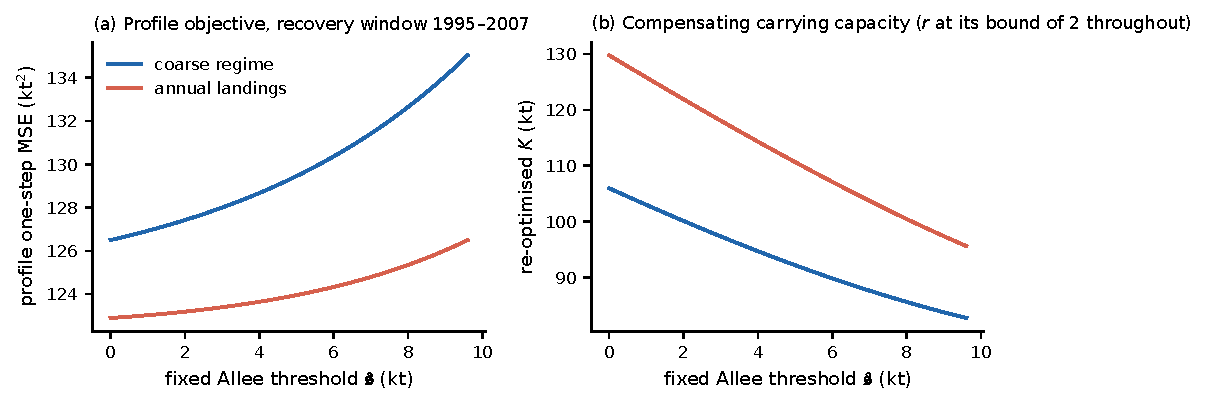
\includegraphics[width=\textwidth]{figS1_allee_profile}
\caption{Profile of the one-step objective over a fixed depensation threshold $\sA$ in the recovery window (train 1995--2007), with $r$ and $K$ re-optimised at each value. (a) The objective rises monotonically from $\sA = 0$ and changes by 6.7\% (coarse regime, 126.5 to 135.0\,kt$^2$) and 2.9\% (annual landings, 122.9 to 126.5) across the range below the smallest observed state (9.7\,kt). (b) The compensating $K$ falls as $\sA$ rises, with $r$ at its bound of 2 throughout. The threshold is unidentified in this window; its least-squares value is the boundary.}
\label{fig:si_profile}
\end{figure}

\FloatBarrier
\section{Floor-forecast census}\label{si:floor}

A forecast is at the floor when the iterated map reaches the numerical floor $\epsilon = 10^{-3}\kt$; its absolute error then equals the observed SSB. Table~\ref{tab:si_floor} counts floor forecasts by band from the archived per-origin files (coarse regime for Specification A). The counts in the first block are those behind the superscripts of Table 6 and Table~\ref{tab:si_h5}.

\begin{table}[!htb]
\centering\small
\caption{Number of origins at which the forecast is at the floor, by band and horizon.}
\label{tab:si_floor}
\begin{tabular}{@{}llrrrrrr@{}}
\toprule
Spec. & Origins & $n$ & M1 & M1b & M2 & M3 & M4 \\
\midrule
A, $h=1$ & 1990--1995 & 6 & 3 & 4 & 0 & 3 & 0 \\
A, $h=1$ & 1996--2012 & 17 & 12 & 13 & 0 & 0 & 0 \\
A, $h=1$ & 2013--2014 & 2 & 0 & 0 & 0 & 0 & 0 \\
A, $h=5$ & 1990--1995 & 6 & 4 & 4 & 1 & 3 & 1 \\
A, $h=5$ & 1996--2010 & 15 & 15 & 15 & 0 & 0 & 0 \\
B, $h=1$ & 1965--1990 & 26 & 2 & 3 & 0 & 0 & 0 \\
B, $h=1$ & 1991--1995 & 5 & 3 & 3 & 0 & 3 & 1 \\
B, $h=1$ & 1996--2012 & 17 & 17 & 17 & 0 & 0 & 0 \\
B, $h=1$ & 2013--2023 & 11 & 0 & 1 & 0 & 0 & 0 \\
B, $h=5$ & 1965--1990 & 26 & 10 & 17 & 7 & 7 & 7 \\
B, $h=5$ & 1991--1995 & 5 & 4 & 5 & 0 & 4 & 3 \\
B, $h=5$ & 1996--2012 & 17 & 17 & 17 & 0 & 0 & 0 \\
B, $h=5$ & 2013--2019 & 7 & 5 & 7 & 0 & 0 & 0 \\
\bottomrule
\end{tabular}
\end{table}

On Specification A the one-step M1 forecast is at the floor at every origin from 1993 to 2007; at 2008--2012 it forecasts 13--37\,kt from states of 91--169\,kt, and at 2013--2014 it forecasts 105 and 204\,kt against 250 and 299. The mechanism is the constant catch: at the 2000 origin the training-mean catch is 129\,kt (coarse) or 122\,kt (annual) against a state of 34\,kt, and at the 2010 origin 85 or 79\,kt against 91\,kt. On Specification B the training-mean catch is 317\,kt at the 1995 origin and still 201\,kt at the 2020 origin.

The log-RMSE diagnostic of the archived summaries uses $\log\max(\hat S,\epsilon)$ and is dominated by these floor forecasts; over the whole origin sets the floor binds for M1 at 15 of 25 ($h=1$) and 19 of 21 ($h=5$) origins on the Specification A annual pass and at 22 of 59 and 36 of 55 on Specification B, for M1b at 17/25, 19/21, 24/59 and 46/55, and for M2--M4 at between zero and eleven origins per cell. The raw RMSE, not the log column, is the retention score.

\FloatBarrier
\section{Secondary scores}\label{si:secondary}

\begin{table}[!htb]
\centering\small
\caption{Brier score of the hard below-threshold indicator implied by the point forecast ($\hat S < $ threshold against $S <$ threshold), origin-matched. Specification A uses the LRP of 884.6\,kt, below which every origin and target after 1990 lies, so the indicator never varies and persistence scores zero trivially; Specification B uses $\Blim = 276\kt$, which the series crosses in 1977, 1980, 1993 and 2016.}
\label{tab:si_brier}
\begin{tabular}{@{}lrrrr@{}}
\toprule
 & A, $h=1$ & A, $h=5$ & B, $h=1$ & B, $h=5$ \\
\midrule
persistence & 0.000 & 0.000 & 0.068 & 0.291 \\
M1 & 0.040 & 0.048 & 0.051 & 0.455 \\
M1b & 0.000 & 0.048 & 0.153 & 0.473 \\
M2 & 0.080 & 0.143 & 0.068 & 0.364 \\
M3 & 0.080 & 0.095 & 0.017 & 0.309 \\
M4 & 0.080 & 0.143 & 0.068 & 0.382 \\
\bottomrule
\end{tabular}
\end{table}

On Specification B the M3 indicator has the lowest one-step Brier score (0.017 against 0.068 for persistence: one misclassified crossing instead of four), and M1's five-year score (0.455) is the worst because it forecasts the floor through two decades in which the stock sat just below $\Blim$ and then crossed it. The direction-of-change score, the fraction of consecutive targets whose observed and forecast changes agree in sign, is 0.80--1.00 for the structural modules on Specification A and undefined for persistence (its forecast change is zero); it separates modules on an outcome that scarcely varies and carries no retention weight.

An interval-scale comparison is available on Specification B because the assessment publishes 95\% limits for its own predictand, with median relative width 0.44. Writing $D = |\hat S_{t+h|t} - S_{t+h}| / [(\mathrm{hi}_{t+h}-\mathrm{lo}_{t+h})/2]$, the proportion of hindcast errors not exceeding half the published width is 56\% for persistence, 36\% for M1 and 59\% for M3 at $h=1$ ($n=59$), and 18\%, 5\% and 7\% at $h=5$ ($n=55$). These are not coverage probabilities: the published interval expresses uncertainty about true biomass given the assessment's data, re-centring its width on a hindcast gives an interval with no established coverage, and the limits are right-skewed on the biomass scale (67 of 71 years asymmetric by more than 10\%). The statistic indicates only that hindcast discrepancies are of the same order as, or larger than, reported target-state uncertainty, and that M3 reads marginally above persistence on it at one step where the RMSE ordering does not.

\FloatBarrier
\section{Simulation: design and full decomposition}\label{si:sim}

\begin{table}[!htb]
\centering\small
\caption{Data-generating processes. All series have $T=33$ years (the Specification A length) with Gaussian process noise $\sigma\in\{11.8, 33.8\}\kt$ entering the state update; parameters are the archived fixed-window fits. Rolling origins use the eight-year minimum training length of Specification A. M3 and M4 were not simulated as truths.}
\label{tab:si_dgp}
\begin{tabularx}{\textwidth}{@{}lLL@{}}
\toprule
DGP & Generating process & Source of parameters \\
\midrule
D1 & M1 autonomous Schaefer, $r=1.935$, $K=1032.7$, $C\equiv 240$, $S_0 = 900$ & collapse-window coarse fit \\
D2 & M1 autonomous Schaefer, $r=0.458$, $K=500$, $C\equiv 5$, $S_0 = 30$ & recovery-window coarse fit \\
D3 & M2 stock-flow, $r=1.935$, $K=1032.7$, catch 240/120/5 along the Specification A schedule, $S_0=900$ & collapse fit and regime path \\
D4 & M1b depensatory, $r=0.458$, $K=500$, $\sA=15$, $C\equiv 5$, $S_0=30$ & recovery fit with an identifiable threshold \\
D5 & Persistence-true null, $S_{t+1} = S_t + \eta_t$, no production, $C\equiv 0$, $S_0=300$ & -- \\
D6 & Drifting productivity, $r_t = 1.935\,e^{-0.05t} + 0.35$, $K=1032.7$, catch 55\% of the instantaneous $r_tK/4$ & Amendment 1 (outside the class) \\
D7 & Smooth path: noise-free state at $r=0.9$, $K=1032.7$, $C=180$, scored series $=$ state plus Gaussian noise & Amendment 1 (outside the class) \\
\bottomrule
\end{tabularx}
\end{table}

The design sheet (\texttt{SPECIFICATION\_v4.md}) was locked at commit \texttt{d5d9758} on 2026-09-10 and the simulation code was written afterwards to implement it; no design element was changed after execution. Amendment 1 (D6, D7, and a $T=71$ series-length cell for D1 and D5) was locked at commit \texttt{bd0008f} on 2026-09-11; the $T=71$ cell was started and abandoned as infeasible (45.6\,s per rolling pass against 7\,s at $T=33$), so no series-length sensitivity is claimed. A module counts as retained in a replicate if it passes (H1)--(H3) at both horizons exactly as in the empirical rule.

\begin{table}[!htb]
\centering\small
\caption{Where the power is lost (averaged over the two noise levels). ``H2 alone'' is the persistence hurdle with the band at both horizons, ignoring the comparator.}
\label{tab:si_power}
\begin{tabular}{@{}llrrrr@{}}
\toprule
DGP & truth & passes H2 alone & passes full rule & removed by comparator & conditional on H2 \\
\midrule
D1 & M1 & 0.975 & 0.975 & 0.000 & 0\% \\
D2 & M1 & 0.420 & 0.420 & 0.000 & 0\% \\
D3 & M2 & 0.328 & 0.100 & 0.228 & 69\% \\
D4 & M1b & 0.180 & 0.010 & 0.170 & 94\% \\
\bottomrule
\end{tabular}
\end{table}

\begin{table}[!htb]
\centering\small
\caption{Chance baseline: proportion of replicates in which the generating module has the lowest one-step RMSE among the five modules (chance $=0.20$).}
\label{tab:si_chance}
\begin{tabular}{@{}lrl@{}}
\toprule
DGP & true module ranks first & against chance \\
\midrule
D1 (M1 true) & 0.627 & far better \\
D2 (M1 true) & 0.645 & far better \\
D3 (M2 true) & 0.038 & worse than chance \\
D4 (M1b true) & 0.258 & barely better \\
\bottomrule
\end{tabular}
\end{table}

In absolute terms the dominant failure is the persistence hurdle: a true module often does not out-predict persistence on data it generated. Conditional on clearing it, the comparator hurdle removes most of the survivors for the stock-flow and depensatory truths. On D3 the stock-flow module's mean one-step error (85.7\,kt) exceeds that of the residual (77.9) and depensatory (79.9) modules, so estimation noise actively disadvantages the correct structure relative to its siblings at this sample size. Under the four structural processes the false-retention rate is 0.044 per module--replicate pair (0.176 falsely retained modules per replicate); under the persistence-true null it is 0.005 per module. Under D6 and D7 the module falsely retained is overwhelmingly M1 (134 and 151 of 200 replicates under D6, 195 and 185 under D7): a constant-productivity map out-predicts persistence on a smoothly drifting or smoothly observed series often enough to clear both hurdles. The alternative decision rules of Table 8 were evaluated on the same archived replicates without refitting.

Two candidate diagnostics for predicting from the data alone whether the rule has power were examined and both fail. The dispersion of scores across modules (median coefficient of variation) correlates with true-module power at Spearman $\rho = 0.52$, too weakly to license a protocol. The margin of the best-scoring module over persistence correlates at $\rho = 0.88$ (Pearson $r = 0.94$) but is computed from the same out-of-sample scores the rule consumes, so it cannot gate the decision, and thresholding it at the tie band misclassifies both D3 cells, flagging ``apply'' where the generating module wins less often than chance. Identifying when the rule has power remains open.

\FloatBarrier
\section{Decomposition of the lagged-start deficit}\label{si:m4}

M4 differs from M3 in two ways: it starts the path from $S_{t-1}$, and it therefore integrates one more catch year. A delayed-persistence control, $\hat S_{t+h} = S_{t-1}$, isolates the information delay. Its one-step RMSE is 184.4\,kt on Specification A and 158.0\,kt on Specification B, against 98.0 and 84.4 for ordinary persistence; the delay alone therefore costs 86.4 of M4's 97.5-kt deficit against persistence on A and 73.6 of 121.3 on B. The lagged start is an information-delay penalty, not a dynamical one, and M4 is not retained for the same reason that a one-year-stale persistence forecast would not be.

\FloatBarrier
\section{The rule applied elsewhere: Edwards Aquifer restatement}\label{si:edwards}

The same retention rule, with the same hurdles, band and horizons, was applied in Abaee (2026, Does a one-pool water-balance model improve forecasts of Edwards Aquifer head) to a one-pool water-balance forecaster of the J-17 index well. There the module's one-step RMSE was 12.84\,ft against 13.23\,ft for persistence, a 2.96\% improvement inside the 5\% band, and at five years the ordering reversed (21.25 against 21.11\,ft). Retention was withheld by the band and the two-horizon requirement. On the cod series no module comes within the band at either horizon, so the ranking alone decides. The two applications share the rule and nothing else; neither series is pooled with the other and no verdict is transferred.
\FloatBarrier
\section{Vintages and thresholds}\label{si:thresholds}

\paragraph{Vintage overlap, 1983--2015} The NCAM Table A2 vintage (Specification A) and the RAM Legacy v4.66 continuation of the same assessment family (stock COD2J3KL) differ over 1983--2015 by $+24.7\kt$ on average (Table A2 higher), by 26.8\,kt in mean absolute value and by 131.2\,kt at most, in 1984 (Fig.~\ref{fig:si_vintages}). The xteNCAM revision differs from Table A2 over the same years by 126.2\,kt RMSE, with Table A2 higher by 58.5\,kt on average. The 2015 origin is 298.65\,kt on Table A2, 277\,kt on RAM and 273\,kt on xteNCAM.

\paragraph{Vintage-shifted LRP} The LRP defined as the 1983--1989 mean is 884.6\,kt on the Table A2 vintage and 790.0\,kt on the RAM vintage, a shift of 94.6\,kt in the reference point from a revision of the same model family. Persistence from the 2015 origin under-predicts every outcome year 2016--2021 in both vintages: MAE 129.2\,kt and RMSE 133.3\,kt from the RAM origin of 277\,kt, MAE 107.5\,kt from the Table A2 origin. The outcome years agree across the RAM and xteNCAM vintages to within 1--26\,kt (mean absolute difference 16.8\,kt).

\paragraph{Threshold classification on one file} The xteNCAM file (1954--2024, 71 years) carries a ratio column that fixes $\Blim$ at 276\,kt (per-year implied values 250--289, mean 275.5). Classifying each year under $\Blim = 276\kt$ and under the 884.6-kt LRP gives 45 years at or above $\Blim$, 16 years at or above the LRP (1954--1969 only), and 29 disagreement years in two blocks: 1970--1992 without 1977--1979, and every outcome year 2016--2024. Under the 1980s-mean threshold the stock stands below the reference point for 55 consecutive years (1970--2024); under $\Blim$ it is below for 26 years (1977--1979 and 1993--2015) and above from 2016 onward. The late-1970s episode (ratios 0.69--0.95) is a critical-zone reading, on the current model, of years the contemporary fishery regarded as healthy. The checkpoints 2005, 2017 and 2024 read 26, 451 and 342\,kt. The October 2023 framework revision, which moved the stock's reported zone from critical to cautious without a change in the stock, is this experiment executed by the assessment authority. The scored RMSE comparison never uses the thresholds; every normative verdict layered on the forecasts, the Brier indicator included, inherits the dependence.

\begin{figure}[!htb]
\centering
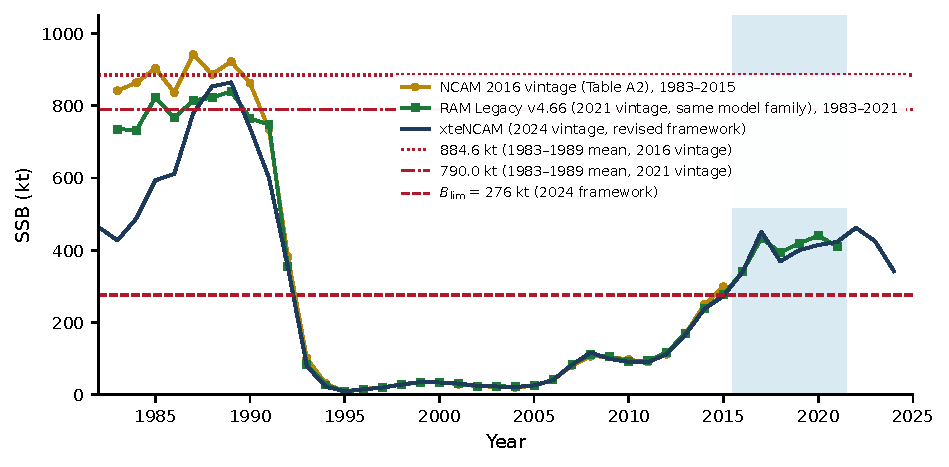
\includegraphics[width=\textwidth]{figS2_vintages}
\caption{Three vintages of Northern cod SSB over 1983--2024: NCAM Table A2 (Specification A, 1983--2015), RAM Legacy v4.66 (the same assessment family continued to 2021) and xteNCAM Table 17 (Specification B). Horizontal lines mark the two Specification A LRP values (884.6\,kt on Table A2, 790.0\,kt on the RAM vintage) and $\Blim = 276\kt$. The outcome years 2016--2021 lie above the 2015 origin in every vintage and below 884.6\,kt in every vintage.}
\label{fig:si_vintages}
\end{figure}

\FloatBarrier
\section{The 2022--2023 observation suspension}\label{si:suspension}

The test conditions on a complete annual series. The stock's real 2022--2023 history violates that condition. Partial coverage by the fall research-vessel survey in 2021 and 2022 left the leading indicator of stock size uncomputable; no typical assessment update was possible in 2022 or 2023; the stewardship maximum was rolled over unchanged at 12{,}999 t; and the survey vessel that carries the series was condemned in February 2023. Table~\ref{tab:si_suspension} assembles the episode from the assessment of record and the public record.

\begin{table}[!htb]
\centering\small
\caption{The 2022--2023 observation suspension and its resolution (sources: Regular et al.\ 2025 and its Table 17 file; the 2024 reopening announcement; the 2025 and 2026 assessment coverage).}
\label{tab:si_suspension}
\begin{tabularx}{\textwidth}{@{}lL@{}}
\toprule
Period & Event \\
\midrule
2021--22 & Partial fall-survey coverage; leading indicator not computable \\
2022--23 & No typical assessment update; stewardship maximum held at 12{,}999 t \\
Feb 2023 & Survey vessel condemned \\
Mar 2024 & Revised-framework assessment: SSB at 1.2 \(B_{\mathrm{lim}}\) (95\% CI 0.7--2.1; 22\% critical-zone probability) \\
Jun 2024 & Commercial fishery reopened at 18{,}000 t after 32 years \\
2025 & TAC 38{,}000 t; reference point revised after being deemed overestimated \\
Apr 2026 & Healthy-zone report: SSB $\approx$ 540 kt (CI 420--700); 70\% probability above the upper stock reference \\
\bottomrule
\end{tabularx}
\end{table}

Read against a review-timing rule under which a review must land no later than the worst-case loss of the information it consumes, the episode is that rule's boundary case in the wild: the information loss ran past the review cadence, and the removals rule froze for two cycles while the observation map was dark. Abaee (2026, Periodic review as sampled governance) states the formal identity; the 2022--2023 suspension is its empirical instance, and it marks the practical limit of any scoring exercise that presumes the series exists.

\FloatBarrier
\section{Reproducibility and verification record}\label{si:repro}

\paragraph{Determinism} All computations are deterministic: within a fixed interpreter and library stack, repeated executions reproduce every result file byte for byte. An independent re-execution verified all 29 recorded output checksums and regenerated all 30 result files byte-identically; one archived file carries no pinned checksum and is covered by the regeneration comparison. Across environments (Python 3.12, numpy 2.1.3, scipy 1.14.1 against the recorded original environment), the intervention runners and the OLS-based prediction runners regenerate their outputs byte for byte, while the four optimiser-based forecast runners (L-BFGS-B fits) reproduce every scored row at printed precision with one exception: the M1b rolling row on Specification B, whose depensatory optimum is environment-sensitive at the $\pm17\kt$ level ($h=1$: 151.6 against 153.2\,kt; $h=5$: 445.5 against 462.5\,kt). That sensitivity is the identification fragility of Section~\ref{si:params} and is immaterial to the verdict, which persistence wins at both horizons by margins far larger than the instability.

\paragraph{Third environment (this revision)} For this revision the four forecast runners (\texttt{run\_ladder.py}, \texttt{run\_xte.py}, \texttt{run\_capelin\_regime.py}, \texttt{run\_capelin\_index.py}), the uncertainty script and the simulation outputs were re-executed or re-read in a third environment (Python 3.13.16, numpy 2.3.5, scipy 1.17.1). Every result file, including the M1b rows, was reproduced at printed precision, and the persistence baselines were recomputed from the series on the archived origin sets and matched the archived origin-matched values (98.05, 264.72, 84.43, 299.98\,kt). The paired block bootstrap was re-run from the archived per-origin files with an explicitly shared index draw and reproduced every interval of Table~\ref{tab:si_dm}. The period decomposition, the rolling parameter record, the floor census and the catch-timing sensitivity were computed in the same environment from the archived files and the unmodified runner functions; their scripts are archived under \texttt{paperE1\_cod\_forecast\_ladder\_v69\_src/work/}.

\paragraph{Verification script} \texttt{paperE1\_cod\_forecast\_ladder\_v69\_verification.py} (standard library only) regenerates every number of Section 4.7 and of Sections~\ref{si:thresholds}--\ref{si:suspension} from the archived data files (NCAM Table A2, RAM v4.66 time series, xteNCAM Table 17, the capelin index) and asserts the cross-checks, including the presence in the manuscript source of the pinned values and the suspension facts. All checks pass on the main text and this document taken together.

\paragraph{Scripts}
\begin{verbatim}
python3 wave_e_cod/src/run_ladder.py
python3 wave_e_cod/src/run_xte.py
python3 wave_e_cod/src/run_capelin_regime.py
python3 wave_e_cod/src/run_capelin_index.py
python3 "batch 7 .../campaign_e1_dm_uncertainty_regime.py"
python3 tools/sim_retention_power.py
python3 paperE1_cod_forecast_ladder_v69_src/work/paired_bootstrap.py
python3 paperE1_cod_forecast_ladder_v69_src/work/post1995.py
python3 paperE1_cod_forecast_ladder_v69_src/work/catch_timing_sensitivity.py
python3 paperE1_cod_forecast_ladder_v69_src/work/make_figures.py
\end{verbatim}

\FloatBarrier
\section{Catch-timing convention: a sensitivity outside the archived protocol}\label{si:timing}

In \texttt{run\_ladder.py} the estimator pairs the increment $S_{j+1}-S_j$ with the catch $C_j$ of the same year, whereas the forecast path at origin $t$ applies $C_{t+1},\dots,C_{t+h}$ to the steps $t\to t+1,\dots,t+h-1\to t+h$. The two conventions differ by one year. The estimation convention is the one under which SSB is a start-of-year quantity and $C_t$ the removals during year $t$; the forecast convention gives the catch-supplied modules the catch of the target year, which under that reading occurs after the predictand is realised. The offset was noticed during the re-execution for this revision. Table~\ref{tab:si_timing} re-runs M2--M4 with the estimation convention in the forecast path (persistence and M1/M1b are unaffected). Under the coarse regime the two conventions differ only at the 1990--1992 origins, where the regime boundaries fall; under annual landings and on Specification B they differ at every origin.

\begin{table}[!htb]
\centering\small
\caption{Rolling-origin RMSE (kt) of the catch-supplied modules under the archived forecast convention ($C_{t+1}$ applied to the step $t\to t+1$) and under the estimation convention ($C_t$), with the ratio to origin-matched persistence in parentheses.}
\label{tab:si_timing}
\begin{tabular}{@{}llcrrr@{}}
\toprule
Spec.\ (catch) & Module & $h$ & archived & estimation convention & persistence \\
\midrule
A annual & M2 & 1 & 160.4 (1.64) & 133.3 (1.36) & 98.0 \\
A annual & M2 & 5 & 393.8 (1.49) & 390.8 (1.48) & 264.7 \\
A annual & M3 & 1 & 153.6 (1.57) & 125.5 (1.28) & 98.0 \\
A annual & M3 & 5 & 351.5 (1.33) & 352.2 (1.33) & 264.7 \\
A annual & M4 & 1 & 206.3 (2.10) & 161.9 (1.65) & 98.0 \\
A annual & M4 & 5 & 486.4 (1.84) & 438.7 (1.66) & 264.7 \\
A coarse & M2 & 1 & 144.1 (1.47) & 113.4 (1.16) & 98.0 \\
A coarse & M2 & 5 & 398.2 (1.50) & 367.8 (1.39) & 264.7 \\
A coarse & M3 & 1 & 134.6 (1.37) & 105.2 (1.07) & 98.0 \\
A coarse & M3 & 5 & 366.4 (1.38) & 341.5 (1.29) & 264.7 \\
A coarse & M4 & 1 & 195.6 (1.99) & 138.9 (1.42) & 98.0 \\
A coarse & M4 & 5 & 488.2 (1.84) & 409.8 (1.55) & 264.7 \\
B & M2 & 1 & 166.0 (1.97) & 146.4 (1.73) & 84.4 \\
B & M2 & 5 & 1058.9 (3.53) & 981.8 (3.27) & 300.0 \\
B & M3 & 1 & 126.7 (1.50) & 94.9 (1.12) & 84.4 \\
B & M3 & 5 & 930.1 (3.10) & 832.5 (2.78) & 300.0 \\
B & M4 & 1 & 205.7 (2.44) & 130.3 (1.54) & 84.4 \\
B & M4 & 5 & 1030.7 (3.44) & 898.3 (2.99) & 300.0 \\
\bottomrule
\end{tabular}
\end{table}

Under the estimation convention every one-step deficit shrinks and no five-year deficit changes sign. M3 is 7\% above persistence at one year on Specification A (coarse) and 12\% on Specification B, still outside the 5\% band, and 29\% and 178\% above at five years. The post-1995 bands of Table 6 are unchanged on Specification A (the catch is constant at 5\,kt there under the coarse regime); on Specification B the post-1995 one-step M3 margin becomes $+10.4\kt$ with interval $[-20.2, +46.8]$ ($p = 0.53$), M2 and M4 remain significantly worse ($+62.0$, $[+24.6, +98.7]$; $+45.9$, $[+11.8, +86.4]$), and all five-year margins remain far outside the band. The verdict of the main text does not depend on the convention; the size of the one-step deficits does, and a future application of the ladder should use the estimation convention throughout.

\begin{figure}[!htb]
\centering
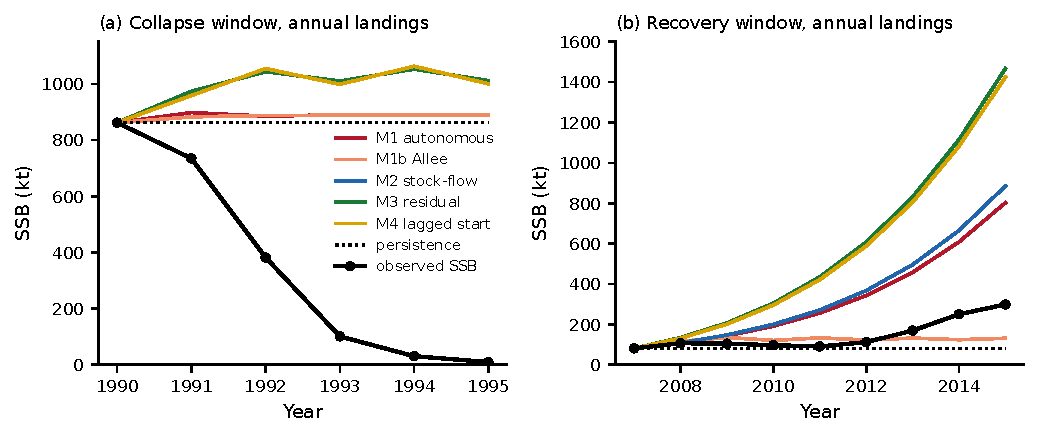
\includegraphics[width=\textwidth]{figS3_windows_annual}
\caption{Fixed-window forecast paths on Specification A with annual landings (companion to Fig.~3). (a) Collapse window: as under the coarse regime, every module forecasts continuation or growth. (b) Recovery window: with $K$ at its 5000-kt bound, production does not saturate and the catch-supplied modules over-predict more than under the coarse regime (M3 609\,kt RMSE against 220); M1b is again a flat line at its fitted $K$.}
\label{fig:si_annual}
\end{figure}

\end{document}
